\begin{figure}[p]
\centering
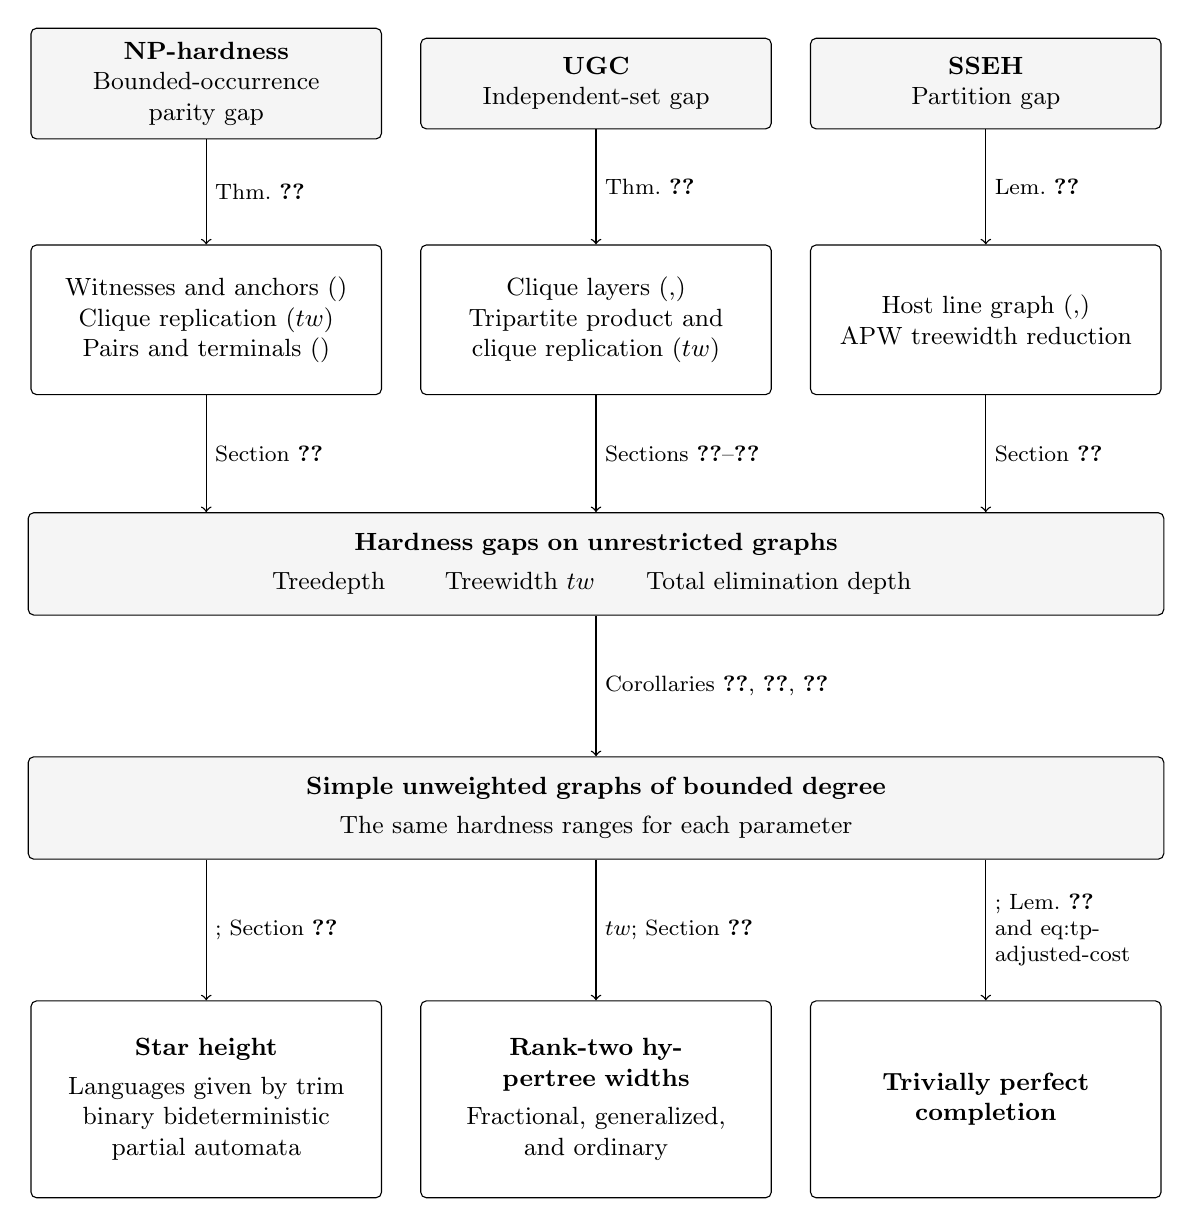
\begin{tikzpicture}[
 x=1cm,y=1cm,font=\small,
 source/.style={draw,rounded corners=2pt,align=center,text width=4.1cm,
   minimum height=1.15cm,inner sep=5pt,fill=black!4},
 construction/.style={draw,rounded corners=2pt,align=center,text width=4.1cm,
   minimum height=1.9cm,inner sep=5pt},
 shared/.style={draw,rounded corners=2pt,align=center,text width=14cm,
   minimum height=1.3cm,inner sep=6pt,fill=black!4},
 application/.style={draw,rounded corners=2pt,align=center,text width=4.1cm,
   minimum height=2.5cm,inner sep=5pt},
 mapref/.style={font=\footnotesize,align=left,inner sep=3pt},
 maparrow/.style={->,line width=.5pt}
]
% Sources and constructions occupy the same three columns throughout.
\node[source] (np-source) at (0,0)
 {\textbf{NP-hardness}\\Bounded-occurrence parity gap};
\node[source] (ugc-source) at (4.95,0)
 {\textbf{UGC}\\Independent-set gap};
\node[source] (sse-source) at (9.9,0)
 {\textbf{SSEH}\\Partition gap};

\node[construction] (np-build) at (0,-3)
 {Witnesses and anchors ($\td$)\\
  Clique replication ($\operatorname{tw}$)\\
  Pairs and terminals ($\totd$)};
\node[construction] (ugc-build) at (4.95,-3)
 {Clique layers ($\td,\totd$)\\
  Tripartite product and\\clique replication ($\operatorname{tw}$)};
\node[construction] (sse-build) at (9.9,-3)
 {Host line graph ($\td,\totd$)\\
  APW treewidth reduction};

\draw[maparrow] (np-source.south) --
 node[mapref,right] {Thm.~\ref{thm:xor-source}} (np-build.north);
\draw[maparrow] (ugc-source.south) --
 node[mapref,right] {Thm.~\ref{thm:bounded-degree-kr-source}} (ugc-build.north);
\draw[maparrow] (sse-source.south) --
 node[mapref,right] {Lem.~\ref{lem:sse-unweighted-gap}} (sse-build.north);

% A shared node bundles the three objectives, rather than their gadgets.
\node[shared] (gaps) at (4.95,-6.1)
 {\textbf{Hardness gaps on unrestricted graphs}\\[3pt]
  Treedepth $\td$\qquad Treewidth $\operatorname{tw}$\qquad
  Total elimination depth $\totd$};
\draw[maparrow] (np-build.south) --
 node[mapref,right] {Section~\ref{sec:np-hardness}}
 (np-build.south |- gaps.north);
\draw[maparrow] (ugc-build.south) --
 node[mapref,right] {Sections~\ref{sec:ugc}--\ref{sec:tw-transfer}}
 (ugc-build.south |- gaps.north);
\draw[maparrow] (sse-build.south) --
 node[mapref,right] {Section~\ref{sec:sseh}}
 (sse-build.south |- gaps.north);

\node[shared] (bounded) at (4.95,-9.2)
 {\textbf{Simple unweighted graphs of bounded degree}\\[3pt]
  The same hardness ranges for each parameter};
\draw[maparrow] (gaps.south) --
 node[mapref,right]
 {Corollaries~\ref{cor:td-bounded-degree}, \ref{cor:tw-bounded-degree},
  \ref{cor:total-depth-bounded-degree}} (bounded.north);

% Each application uses the parameter indicated on its incoming edge.
\node[application] (star-height) at (0,-12.9)
 {\textbf{Star height}\\[3pt]
  Languages given by trim\\binary bideterministic\\partial automata};
\node[application] (hypertree) at (4.95,-12.9)
 {\textbf{Rank-two hypertree widths}\\[3pt]
  Fractional, generalized,\\and ordinary};
\node[application] (completion) at (9.9,-12.9)
 {\textbf{Trivially perfect}\\\textbf{completion}};
\draw[maparrow] (star-height.north |- bounded.south) --
 node[mapref,right] {$\td$; Section~\ref{subsec:established-transfers}}
 (star-height.north);
\draw[maparrow] (hypertree.north |- bounded.south) --
 node[mapref,right] {$\operatorname{tw}$; Section~\ref{subsec:established-transfers}}
 (hypertree.north);
\draw[maparrow] (completion.north |- bounded.south) --
 node[mapref,right,text width=2.0cm]
 {$\totd$; Lem.~\ref{lem:tp-fill-depth}\\and~\eqref{eq:tp-adjusted-cost}}
 (completion.north);
\end{tikzpicture}

\medskip
\begin{minipage}{\textwidth}\footnotesize
The hardness ranges are listed in the introduction's table. The degree
bound depends only on the fixed excluded approximation factor.
Each application branch uses its indicated parameter under all three
hardness assumptions.
The SSE treewidth route uses~\cite{APW} and its bounded-degree transfer
in Corollary~\ref{cor:tw-bounded-degree}.
\end{minipage}
\caption{The main reduction routes. Each source column contains the
constructions for the three parameters; the lower branches show three
applications. Further applications appear in Section~\ref{sec:applications}.}
\label{fig:introduction-reduction-map}
\end{figure}
